\documentclass[a4paper]{article}

\usepackage[english]{babel}
\usepackage[utf8x]{inputenc}
\usepackage{graphicx}
\usepackage[colorinlistoftodos]{todonotes}
\usepackage{tabularx}
\usepackage{amsmath}
\usepackage{amssymb}
\usepackage{amsfonts}
\usepackage{adjustbox,lipsum}
\usepackage{fullpage}
\usepackage{times}
\usepackage{fancyhdr,graphicx,amsmath,amssymb}
\usepackage[ruled,vlined]{algorithm2e}
\usepackage{url}
\usepackage{multirow}



\usepackage{caption}
\usepackage{subcaption}
\usepackage{float}

\title{Distributed SNN Clustering for large document collections}

\newcommand{\set}[1]{\mathcal{#1}}
\newcommand*\pct{\scalebox{.9}{\%}}

\SetKwInput{KwData}{Input}
\SetKwInput{KwResult}{Output}

\begin{document}
\maketitle

\begin{abstract}
Your abstract.
\end{abstract}

\section{Introduction}
As a consequence of the explosive growth of the WEB, the integration of search engines such as Google into personal computers and mobile devices, and the wide use of social networks, the task of clustering text data, i.e. Tweets or documents in a search engine, has each time an increasing importance because of the necessity of unraveling the underlying categories in large volumes of text data. Nowadays the generation of large amounts of documents surpasses the computational power of personal computers and even of high performance computers.
As an example, it is estimated that the amount of WEB pages that popular search engines such as Yahoo! and Google index is higher than the tens of a billion \cite{www}.
It is therefore of great interest to develop algorithmic techniques capable of automatically organize, classify and summarize document collections distributed in multiple machines of a network, and that also perform efficiently in modern hardware, particularly within parallel processing frameworks in multi-core architectures. In real problems such as \textit{Collection Selection} for distributed document databases, in which for a given query the computer node containing the most suitable sub-collection must be selected to answer it \cite{CM13}, the challenges related to the scalability and efficiency of \textit{Knowledge Discovery} methods have become very important. Traditional algorithms often assume that the whole dataset is loaded into main memory (RAM) and thus every document can be accessed at any time with no access latency. In scenarios where the size of the collection is much bigger than the amount of available RAM either because of the number of documents or the length of each document, this ideal loading process is unfeasible due to real constraints in the storage or computational capabilities.


Often, text data is structured in digital collections of documents whose length (number of characters) is variable, e.g. WEB pages or the content generated by users in social networks such as Twitter or Facebook. In order to enable the processing of these collections, in a first stage of preprocessing a set of words occurring in the documents are extracted and sorted in lexicographical order; this word set is referred to as the Vocabulary. Then, the content of every document in the collection is represented as a vector in which each dimension denotes a specific word of the Vocabulary and its value in a document vector is given by a function of the number of occurrences of the word within the document and the number of documents in which it appears. As a natural consequence of the lexical richness of every language, the size of the Vocabulary, and in turn the dimensionality of the vector space onto which a document is represented,  is far bigger than the data size that traditional clustering algorithms manage. Because of this, the task of automatic document clustering has high computational and storage (RAM and secondary memory) costs. Along with this, when the number of documents is large (tens or hundreds of thousand and even millions of items) then traditional techniques for processing and clustering documents, and current computational capabilities of a single machine and also high performance machines are insufficient. Even in the most favorable scenario the storage and computational power tackle the challenge but the response time are excessive.


There exist three approaches successfully applied to the construction of clustering algorithms capable of processing large volumes of data. The first one introduces constraints on the number of passes allowed on a document (related to the amount of time it is loaded into main memory) \cite{Yi14, I14}. The second one exploits current multi-core architectures to perform parallel processing of the data, which does not solve the massive volume problem \cite{ZW13}. The last one combines the computational power of a single machine together with the scalable storage capability of a distributed system by partitioning the dataset into several independent machines connected through a network \cite{SC16}.


The last above mentioned approach seems promising since it allows to exploit the local capabilities of single computers with multi-core architectures without sacrificing scalability to large data volumes because of its distributed design. Within this path there are two contexts regarding the data generation scenario. On the one hand, in some problems where the dataset is large but collected in a centralized fashion, the strategy employed consists in partitioning the collection into several machines or nodes of a network. This scheme leads to the transmission of a lot of data during the execution of the algorithm \cite{N15}. On the other hand, there are some problems where the data is generated in a distributed fashion and where besides it is not feasible to centralize the data because of high transmission costs or privacy issues \cite{JW05,LHLX12}, e.g. search engines work with document collections originated and stored in different geographical locations.
%\subsection*{Outline}

This document is structured as follows: First, a review of the literature on scalable and distributed data clustering methods is presented. Next, the proposed method is shown. Finally,the experimental design along with the attained results and the final remarks are presented. 

\section{Distributed Clustering Algorithms}
As far as we know from the literature, most of the existing efforts for the construction of clustering techniques capable of operating in scenarios where the data is distributed have been focused on low dimensional data (less than 100 attributes) in contrast with document datasets in which a document vector for a small collection may have about $10^4$ attributes. Nevertheless, the main advances in distributed data clustering are detailed below, specially highlighting those contributions focused on methods capable of dealing with high dimensional data.


\subsection{Main contributions on parallel algorithms}

In \cite{XJK99}  a parallel version of DBSCAN algorithm is presented (PDBSCAN). The authors present the ‘shared-nothing’ architecture with multiple computers interconnected through a network. A fundamental component of a shared-nothing system is its distributed data structure. They introduce the dR*-tree, a distributed spatial index structure in which the data is spread among multiple computers and the indexes of the data are replicated on every computer. A performance evaluation shows that PDBSCAN offers nearly linear speedup and has excellent scaleup and sizeup behavior. The authors in \cite{DM99} present an algorithm that exploits the inherent data-parallelism in the kmeans algorithm. They analytically show that the speedup and the scaleup of our algorithm approach the optimal as the number of data points increases. The implementation of this proposal is done on an IBM POWERparallel SP2 with a maximum of 16 nodes. On typical test data sets, nearly linear relative speedups are observed, for example, 15.62 on 16 nodes, and essentially linear scaleup in the size of the data set and in the number of clusters desired. For a 2 gigabyte test data set, the implementation drives the 16 node SP2 at more than 1.8 gigaflops.
Another scalable approach based on secondary memory consists in designing algorithms capable of working within the MapReduce framework\footnote{Hadoop MapReduce is a software solution that enables the construction of applications capable of processing large amounts of data (e.g. Terabytes) in a parallel fashion over big computer clusters.}. In this context it is possible to highlight the contributions made by \cite{DDGR07} in which they propose an implementation of the EM algorithm and also by \cite{EIM11} in which they tackle the K-Median problem by using MapReduce.
In \cite{DDGR07} the authors present an approach to filter recommendations for users of Google News in order to generate personalized recommendations in a collaborative way. They generate recommendations using three approaches: collaborative filtering using MinHash clustering, Probabilistic Latent Semantic Indexing (PLSI), and covisitation counts. The recommendations are combined from different algorithms using a linear model. The authors claim that the approach is content agnostic and consequently domain independent, making it easily adaptable for other applications and languages with minimal effort. In \cite{EIM11} the authors design clustering algorithms that can be used in MapReduce, still one of the most popular programming environment for processing large datasets. They focus on the practical and popular clustering problems, k-center and k-median. A fast clustering algorithms with constant factor approximation guarantees is developed. The algorithms use sampling to decrease the data size and they run a time consuming clustering algorithm such as local search or Lloyd's algorithm on the resulting data set. The proposed algorithms have sufficient flexibility to be used in practice since they run in a constant number of MapReduce rounds.  The experiments in the paper show that proposed algorithms' solutions are similar to or better than the other algorithms' solutions.
Another parallel approach for K-Means is presented by \cite{BMVKV12} and it is called K-Means$++$. The initialization of the k means algorithm is crucial, and the authors claim that the proposed algorithm obtains an initial set of centers that is provably close to the optimum solution. A major downside of the k-means++ is its inherent sequential nature, which limits its applicability to massive data: one must make k passes over the data to find a good initial set of centers. In this work the authors show how to drastically reduce the number of passes needed to obtain, in parallel, a good initialization. This is unlike prevailing efforts on parallelizing k-means that have mostly focused on the post-initialization phases of k-means. The proposed initialization algorithm k-means|| obtains a nearly optimal solution after a logarithmic number of passes, and then shows that in practice a constant number of passes suffices. 

Additionally, the EM-Tree proposed by \cite{VVGN15} is very interesting since it allows to process very large datasets, specifically the authors show that it can handle hundred of millions of WEB pages. They present a scalable algorithm that clusters hundreds of millions of web pages into hundreds of thousands of clusters. It does this on a single mid-range machine using efficient algorithms and compressed document representations. It is applied to two web-scale crawls covering tens of terabytes. ClueWeb09 and ClueWeb12 contain 500 and 733 million web pages and were clustered into 500,000 to 700,000 clusters. Previous approaches clustered a sample that limits the maximum number of discoverable clusters. The proposed EM-tree algorithm uses the entire collection in clustering and produces several orders of magnitude more clusters than the existing algorithms. Fine grained clustering is necessary for meaningful clustering in massive collections where the number of distinct topics grows linearly with collection size. These fine-grained clusters show an improved cluster quality when assessed with two novel evaluations using ad hoc search relevance judgments and spam classifications for external validation. These evaluations solve the problem of assessing the quality of clusters where categorical labeling is unavailable and unfeasible.

\subsection{Approaches capable of dealing with high dimensional data} 
\cite{KHSJ01} propose a method to obtain the Principal Components (PCA) over heterogeneous and distributed data. Based on this contribution on dimensionality reduction they also propose a clustering method that works over high dimensional data. Once the global principal components are obtained by using the distributed method and transmitted to each node, local data are projected onto the components and then a traditional clustering technique is applied. Finally, a central node integrates the local clusters in order to obtain a global clustering model.

Several years later, \cite{LBK13} present another algorithm for principal components extraction over distributed data. To this end, each node computes PCA over its local data and transmit a fraction of them to a central node. This node uses the received components to estimate the global principal components, which are later transmitted to each node. After this, in every node, local data are projected onto the global components and the projected data are used for computing a coreset by means of a distributed algorithm. The global coreset built from the local projected data will be finally used to obtain a global clustering model.  

The authors in \cite{LZO03} propose an algorithm called the CoFD algorithm, which is a non-distance based clustering algorithm for high dimensional spaces. Based on the Maximum Likelihood Principle, CoFD attempts to optimize its parameter settings to maximize the likelihood between data points and the model generated by the parameters. The distributed versions of the problem, called the D-CoFD algorithms, are also proposed. The authors claim that the experimental results on both synthetic and real data sets show the efficiency and effectiveness of CoFD and D-CoFD algorithms.

\subsection{Density based approaches}
\cite{JKP03} propose a distributed data clustering technique in which local nodes build models and transmit a set of representatives of each cluster to a central node. In this node a centralized clustering method is applied over the representatives and then the resulting model is re-transmitted to the local nodes to update their models.

In \cite{KLM03} a novel distributed clustering algorithm based on non-parametric kernel density estimation is presented, which takes into account the issues of privacy and communication costs that arise in a distributed environment. They state that several approaches to knowledge discovery and data mining, and in particular to clustering, have been developed, but only a few of them are designed for distributed data sources.

\cite{JKP04} present a scalable version of DBSCAN that is also capable of operating over distributed collections. First, the best local representatives a selected depending on the number of points that each one represents and then those chosen points are sent to a central node. This central node clusters the received local representatives into a single new model, which is re-transmitted to the other nodes so they can improve their local group structure.


\subsection{Approaches based on parametric models}
In \cite{MG03} a framework for clustering distributed data in unsupervised and semisupervised scenarios is proposed, taking into account several requirements, such as privacy and communication costs. Instead of sharing portions of the original data, the authors transmit the parameters of suitable generative models built at each local data site to a central location. They mathematically show that the best representative of all the data is a certain "mean" model, and empirically show that this model can be approximated quite well by generating artificial samples from the underlying distributions using Markov Chain Monte Carlo techniques, and then fitting a combined global model with a chosen parametric form to these samples. Also a new measure that quantifies privacy based on information theoretic concepts is proposed, and it shows that decreasing privacy leads to a higher quality of the combined model and vice versa. They provide empirical results on different data types to highlight the generality of our framework. The results show that high quality distributed clustering can be achieved with little privacy loss and low communication cost.

The authors in \cite{KKPS05} propose a distributed model-based clustering algorithm that uses EM for detecting local models in terms of mixtures of Gaussian distributions.They present an efficient and effective algorithm for deriving and merging these local Gaussian distributions to generate a meaningful global model. In a broad experimental evaluation they demonstrate that the framework is scalable in a highly distributed environment.


\subsection{Approaches based on representative points}


Several works has been proposed over the years that are based on representative points. 
The authors in \cite{FZ00} describe a technique for parallelizing a family of center-based data clustering algorithms. The central idea of the proposed algorithm is to communicate only sufficient statistics, yielding linear speed-up with good efficiency. The proposed technique does not involve approximation and may be used orthogonally in conjunction with sampling or aggregation-based methods, such as BIRCH, to lessen the quality degradation of their approximation or to handle larger data sets. In this paper it is demonstrated that even for relatively small problem sizes, it can be more cost effective to cluster the data in-place using an exact distributed algorithm than to collect the data in one central location for clustering.

\cite{ZLW08} propose an approximate K-Median clustering technique that works over streaming data, i.e. data is continuously collected. They propose a suite of algorithms for computing (1 + $\epsilon$ )-approximate k-median clustering over distributed data streams under three different topology settings: topology-oblivious, height-aware, and path-aware. The proposed algorithms reduce the maximum per node transmission to $polylog N$ (opposed to $\Omega(N)$ for transmitting the raw data). The authors perform simulations on a distributed stream system with both real and synthetic datasets composed of millions of data. In practice, the algorithms are able to reduce the data transmission to a small fraction of the original data. The results indicate that the algorithms are scalable with respect to the data volume, approximation factor, and the number of sites.

\cite{BEL13} address the distributed clustering problem by using centroid based techniques that use a novel coreset construction method that works for distributed data. It provides novel algorithms for distributed clustering for two popular center-based objectives, k-median and k-means. These algorithms have provable guarantees and improve communication complexity over existing approaches. The proposed algorithm reduces the problem of finding a clustering with low cost to the problem of finding a coreset of small size. The authors provide a distributed method for constructing a global coreset which improves over the previous methods by reducing the communication complexity, and which works over general communication topologies. Experimental results on large scale data sets show that this approach outperforms other coreset-based distributed clustering algorithms.

\cite{NC14} tackle the problem of the parameter selection of the K-Means clustering algorithm by using evolutionary algorithms. Two different distribution approaches are adopted: the first obtains a final model identical to the centralized version of the clustering algorithm; the second generates and selects clusters for each distributed data subset and combines them afterwards. The algorithms are compared experimentally from two perspectives: the theoretical one, through asymptotic complexity analyses; and the experimental one, through a comparative evaluation of results obtained from a collection of experiments and statistical tests. The obtained results indicate which variant is more adequate for each application scenario.

\subsection{Hierarchical clustering approaches}

A hierarchical algorithm that works on distributed and heterogeneous data is presented by \cite{JK00}.  This paper presents the Collective Hierarchical Clustering (CHC) algorithm for analyzing distributed, heterogeneous data. This algorithm first generates local cluster models and then combines them to generate the global cluster model of the data. The proposed algorithm runs in $O(|S|n^2)$ time, with a $O(|S|n)$ space requirement and $O(n)$ communication requirement, where $n$ is the number of elements in the data set and $|S|$ is the number of data sites. This approach shows significant improvement over naive methods with $O(n^2)$ communication costs in the case that the entire distance matrix is transmitted and $O(nm)$ communication costs to centralize the data, where m is the total number of features. A specific implementation based on the single link clustering and results comparing its performance with that of a centralized clustering algorithm are presented. An analysis of the algorithm complexity, in terms of overall computation time and communication requirements, is presented.

\cite{JCHAC15} propose a hierarchical clustering algorithm for distributed data that builds the clusters by incrementally processing the data points. The authors re-state the hierarchical clustering problem as a Minimum Spanning Tree construction problem over a graph. In order to integrate several local models they also propose a technique for combining multiple minimum spanning trees, assuming that these trees were obtained from disjoint subgraphs of the complete original graph. This mixture procedure iterates until a single tree is obtained, which in turn denotes the hierarchical clustering originally pursued. 

\section{Proposal}
% Clustering can be used to reduce the amount of data and to induce a categorization
%The goal of clustering is to reduce the amount of data by categorizing or grouping similar data items together
% Illustrate the structure of a given dataset
In this work we present a distributed clustering algorithm based on \textit{Shared-Nearest-Neighbor} (SNN) clustering. This method automatically identifies the number of  underlying groups along with a set of representative points for each one.
We pose that this method is able to deal with collections arbitrarily distributed across a Master/Worker architecture as depicted in figure \ref{fig:distributed_architecture} and the overall algorithm operates in two stages: The first one starts when the data is randomly partitioned and distributed into several nodes, then each one generates a set of representative points per cluster, i.e. \textit{core-points}, and finally, transmits back a sample set of these \textit{core-points} to the master node. In the second stage, the central node joins the sample points received and then starts a centralized SNN clustering over them. Finally, the set of representative points is labeled and also a new set of \textit{core-points} that summarizes the overall collection is obtained.  

\begin{figure}[!htbp]
\centering
  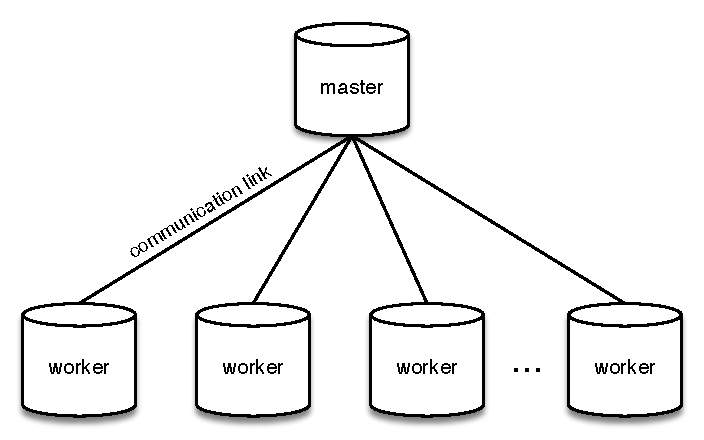
\includegraphics[scale=0.8]{distributed_architecture.pdf}
  \caption{Network architecture employed by the proposed algorithm}
  \label{fig:distributed_architecture}
\end{figure}


%about the parameters
\subsection*{Parameters of the algorithm}
The proposed method comprehends three parameters, namely $k$, $\mathsf{Eps}$, $\mathsf{MinPts}$ and $\omega$. The value of parameter $k$ determines the size of the neighborhood over which the SNN similarity measure is going to be computed. In the SNN space, the value of $\mathsf{Eps}$ denotes the similarity threshold beyond which two points are considered as close. Additionally, a point is identified as a \textit{core-point} when the number of points close to it in the SNN space surpasses the value of parameter $\mathsf{MinPts}$. Finally, the value of the  parameter $\omega$ rules the size of the sample set of \textit{core-points} that is going to be transmitted.

\subsection*{Initial stage}
This stage starts by randomly partitioning and distributing the dataset into several worker nodes.
In this primary stage, after a worker node $n_i$ receives its data chunk $\mathcal{D}_i$, it starts to identify the core-points by following procedure $\mathsf{SnnCorePoints}$ described in algorithm \ref{alg:snncorepointid}. 
Once its core-point set $\mathcal{C}_i$ is built, an attempt to assign a cluster label to each point $p\in \mathcal{C}_i$ is performed.

%\subsubsection*{Labeling step}
Initially, all points are unlabeled. Then, iteratively, each point $p$ is tagged with a new cluster label $l_p$ and subsequently all remaining points located within a radius of $\mathsf{Eps}$ from $p$ in the SNN space are labeled with $l_p$.

Once all core-points are labeled, a weighted sample from each cluster is drawn. The weight of a point follows the expression:\[\dfrac{1 - ( N_l/N_c ) }{2\cdot N_l}\] where $N_c$ denotes the number of labeled core-points and $N_l$ the number of points labeled with label $l$. The expression shown above denotes that the sampling weight of a core-point is inverse to its group size as it is depicted in figure \ref{fig:group_weight}. The aim of this expression is to build a sample of core-points capable of representing both small and large groups alike without a bias to larger clusters which is a serious problem for clustering algorithms operating under unbalanced data scenarios.
The overall procedure is described in algorithm \ref{alg:coresample}. 

\begin{figure}[!htbp]
\centering
  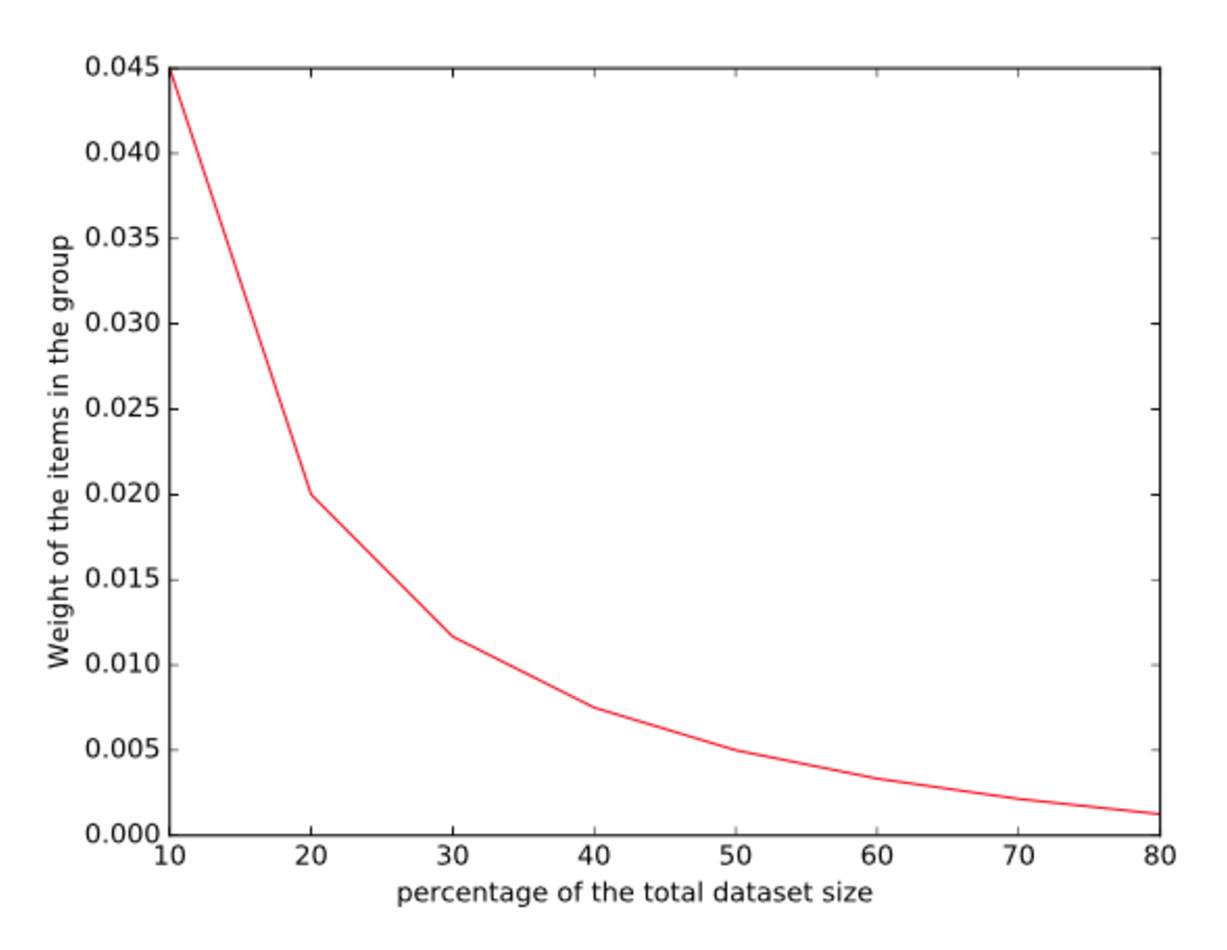
\includegraphics[scale=0.6]{group_weights.pdf}
  \caption{Weight of each item in a group vs the relative size of the group in comparison with the total dataset size.}
  \label{fig:group_weight}
\end{figure}



%\subsubsection*{Identification of core-points}
% TODO: no se que poner aqui aun!!
\subsection*{Final stage}
This stage starts when all worker nodes transmit their weighted sample of core-points to the master node and then this node joins all these points into a single dataset $\mathcal{S}$. 
%As this overall sample contains $\omega[\pct]$ of the dataset, its processing cost is much smaller than the one involved in processing the complete collection. 
Then the procedure $\mathsf{SnnCorePoints}$ is applied over $\mathcal{S}$, obtaining a new core-point set $\mathcal{C}$, and the same labeling step applied in the initial stage in each worker is performed over this set. After this step, for each point $q\in\mathcal{S}$ not chosen for the core-point set $\mathcal{C}$, its nearest neighbor  $p\in\mathcal{C}$ is found. If the SNN similarity between these points is lower than $\mathsf{Eps}$, then $q$ is marked as noise, otherwise label $l_p$ is assigned to $q$.
Finally, the set of labeled points in $\mathcal{S}$ (i.e. discarding the noisy subset) is returned.
A thorough description appears in algorithm \ref{alg:centralproc}.

%algorithms
\begin{algorithm}[!htbp]
   \DontPrintSemicolon
  \SetKwFunction{snncpts}{SnnCorePoints}
  \SetKwProg{Fn}{Function}{:}{}
  
  \Fn{\snncpts{$\mathcal{D}$, $k$, $\mathsf{Eps}$, $\mathsf{MinPts}$}}{
  \ForEach{$p\in\mathcal{D}$}{compute $KNN_{k}(p)$\;}
  \ForEach{$p\in \mathcal{D}$}{
  	\ForEach{$q\neq p\in \mathcal{D}$}{
		$\mathsf{SNN}_{k}(p,q)\leftarrow \#(KNN_{k}(p)\cap KNN_{k}(q))$\; 
    }
    $\mathsf{density}(p)\leftarrow \#\{q\neq p\in\mathcal{D} |\mathsf{SNN}_{k}(p,q)>\mathsf{Eps}\}$\;
    \lIf{$\mathsf{density}(p)>\mathsf{MinPts}$}{Mark $p$ as \textbf{core-point}}
  }
$\mathcal{C}\leftarrow$ all points marked as  \textbf{core-point}\;
\KwRet $\mathcal{C}$ , $\mathsf{SNN}_{k}$\;
  }
\caption{Identification of core-points from a dataset}
\label{alg:snncorepointid}
\end{algorithm}

%node
\begin{algorithm}[!htbp]
% \KwData{$\mathcal{D}$ denotes the local subset of the data, $k$, $\mathsf{Eps}$, $\mathsf{MinPts}$, $\omega\in [0,1]$}
% \KwResult{List of representative points per group}
 \DontPrintSemicolon
  \SetKwFunction{sampleld}{SampleLocalData}
  \SetKwProg{Fn}{Function}{:}{}
  
  \Fn{\sampleld{$\mathcal{D}$, $k$, $\mathsf{Eps}$, $\mathsf{MinPts}$, $\omega\in [0,1]$}}{
  
  $\mathcal{C},\mathsf{SNN}_k\leftarrow$ \snncpts{$\mathcal{D}$, $k$, $\mathsf{Eps}$, $\mathsf{MinPts}$}\;
  
 \ForEach{\bf{core-point} $p\in \mathcal{C}$}{
 	\If{$p$ is not visited}{
    	Assign a new cluster label $l_p$ to $p$\;
	mark $p$ as visited\;
    	\ForEach{Not visited $q\neq p\in\mathcal{C}$}{
        	\If{$\mathsf{SNN}_{k}(p,q)>\mathsf{Eps}$}{
            	Assign label $l_p$ to $q$\;
		mark $q$ as visited\;
            }
    	}
    }    
}
 $N_c\leftarrow$Number of labeled \bf{core-points}\;
 $S\leftarrow\emptyset$\;
 \ForEach{cluster $l$ having size $N_l$}{
 	$S\leftarrow$ Add $\omega\cdot N_l$ points sampled from group $l$ with weight $\dfrac{1 - ( N_l/N_c ) }{2\cdot N_l}$\;
 }
 \KwRet sampled data $S$\;%en L124 se ejecuta el cludtering sobre los datos centralizados.
 }
\caption{Selection of representative points executed in a node}
 \label{alg:coresample}
\end{algorithm}

%central
\begin{algorithm}[!htbp]
 \DontPrintSemicolon
\SetFillComment
\SetKwFor{ForEach}{On each}{execute}{endfch}
\KwData{$\mathcal{D}$ denotes the local subset of the data, $k$, $\mathsf{Eps}$, $\mathsf{MinPts}$, $\omega\in [0,1]$}
%\KwResult{List of representative points per group}
Partition the dataset $\mathcal{D}$ into $M$ subsets $\{D_1, D_2, \ldots D_M\}$\;
\ForEach{node $n_i$}{
	$S_i\leftarrow$ \sampleld{$D_i$}\tcc{remote procedure call on node $n_i$}
}
$S\leftarrow [S_1,S_2,\ldots S_M]$\;
$\mathcal{C},\mathsf{SNN}_k\leftarrow$ \snncpts{$\mathcal{S}$, $k$, $\mathsf{Eps}$, $\mathsf{MinPts}$}\;
\SetKwFor{ForEach}{foreach}{do}{endfch}
 \ForEach{\bf{core-point} $p\in \mathcal{C}$}{
 	\If{$p$ is not visited}{
    	Assign a new cluster label $l_p$ to $p$\;
	mark $p$ as visited\;
    	\ForEach{Not visited $q\neq p\in\mathcal{C}$}{
        		\If{$\mathsf{SNN}_{k}(p,q)>\mathsf{Eps}$}{
        	    		Assign label $l_p$ to $q$\;
			mark $q$ as visited
        		}
    	}
    }    
}

\ForEach{p $\in S\setminus \mathcal{C}$}{
	$n_p\leftarrow \operatorname*{arg\,max}_{q\in \mathcal{C}} \mathsf{SNN}_{k}(p,q)$\;
	\lIf{$\mathsf{SNN}_{k}(p,n_p)<\mathsf{Eps}$}{
		Mark $p$ as \textbf{noise}
	}
	\lElse{
		Assign label $l_{n_q}$ to $p$
	}
}
%Labeled points in $\mathcal{S} Final set of points\;
\KwResult{$\{l_p, p\in S\ |\ l_p\neq \mbox{\textbf{noise}}\}$}  
\caption{Procedure executed by the master node to generate the list of representative points per group}
\label{alg:centralproc}
\end{algorithm}


%TOYEXAMPLE
\begin{figure}[!htbp]
\centering
  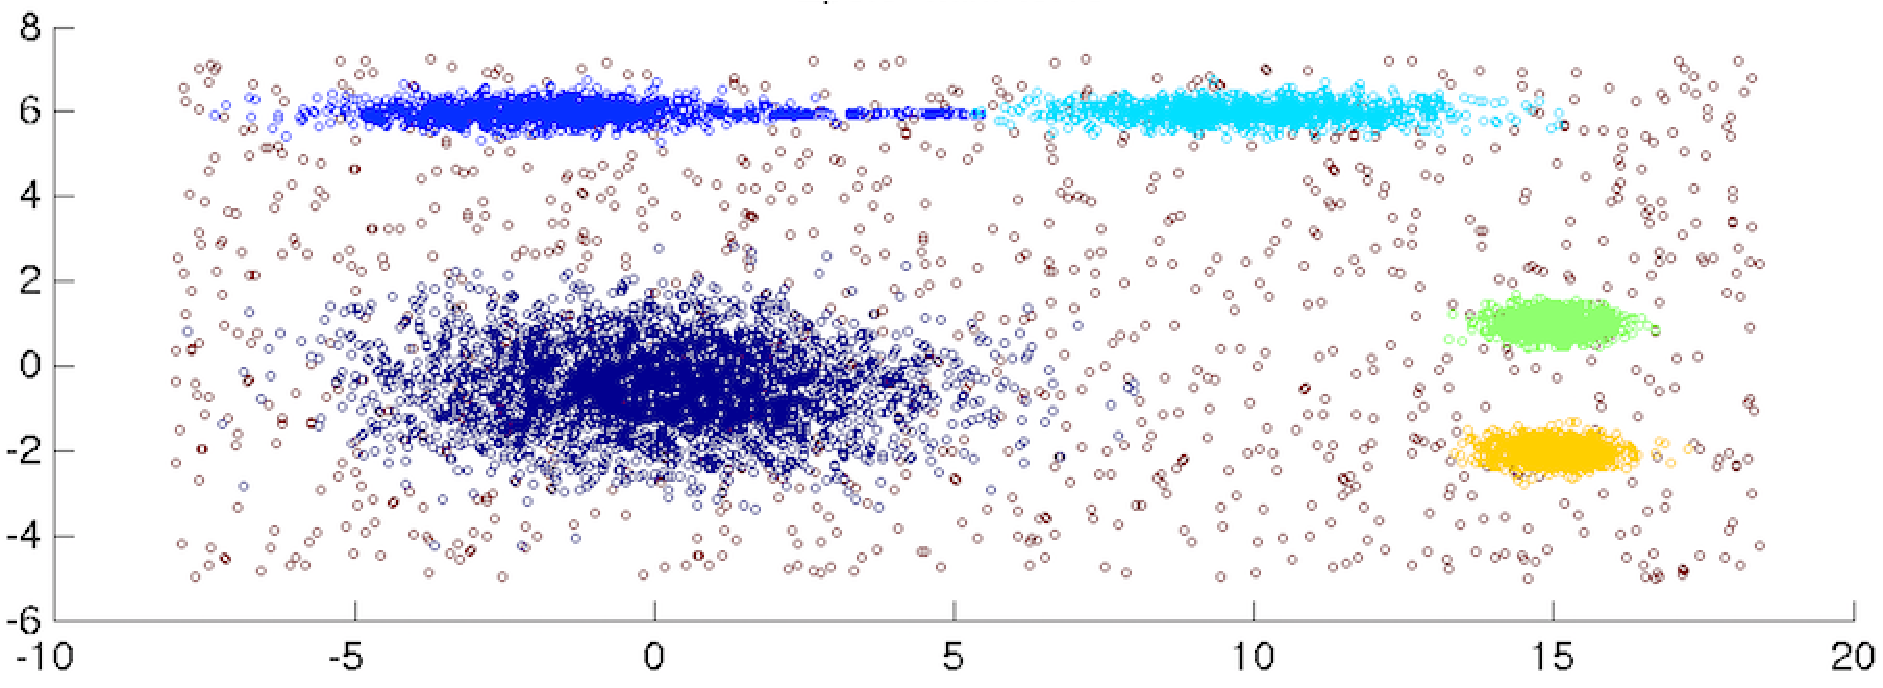
\includegraphics[scale=0.45]
  {toy_example_original.pdf}
  \caption{Toy example: Original data.}
  \label{fig:toy_original}
\end{figure}

\begin{figure}[!htbp]
\centering
  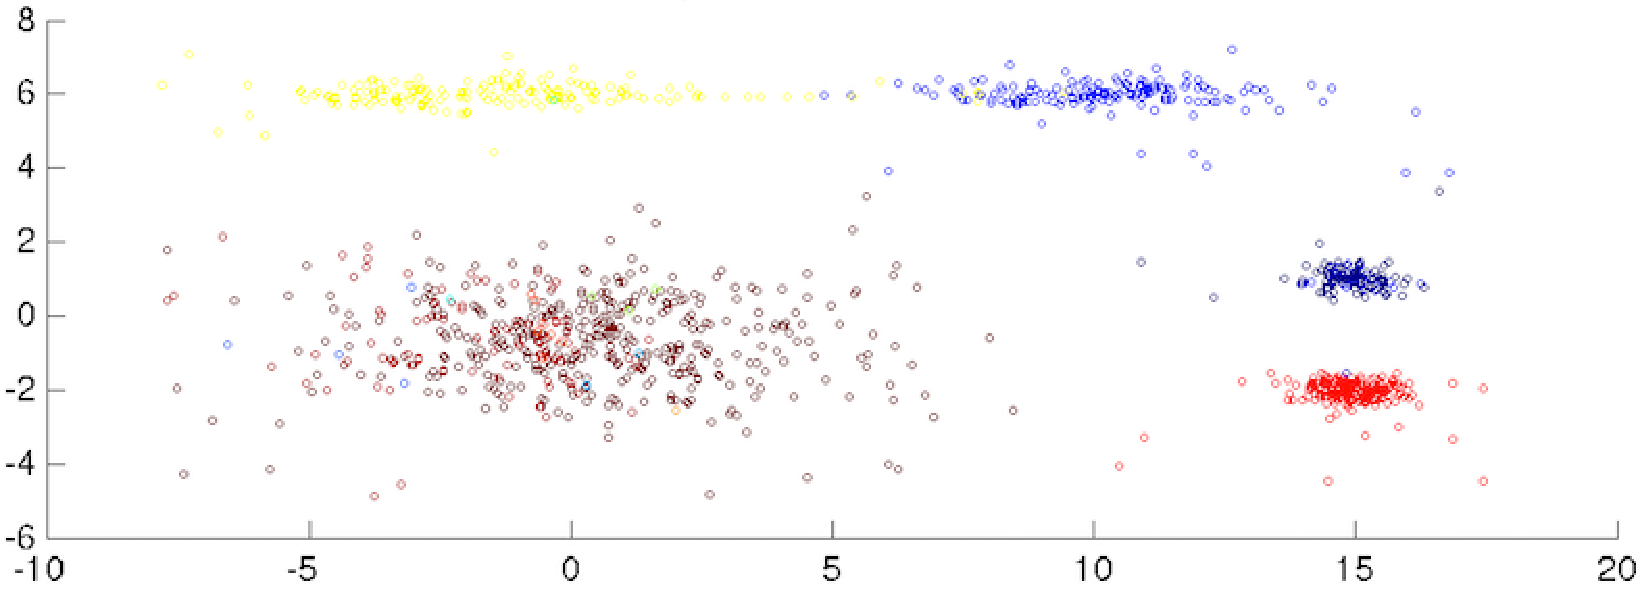
\includegraphics[scale=0.5]{toy_example_after_Dsnn_2.pdf}
  \caption{Toy example: Data after distributed snn clustering with $Eps=50$.}
  \label{fig:toy_dsnn1}
\end{figure}

\begin{figure}[!htbp]
\centering
  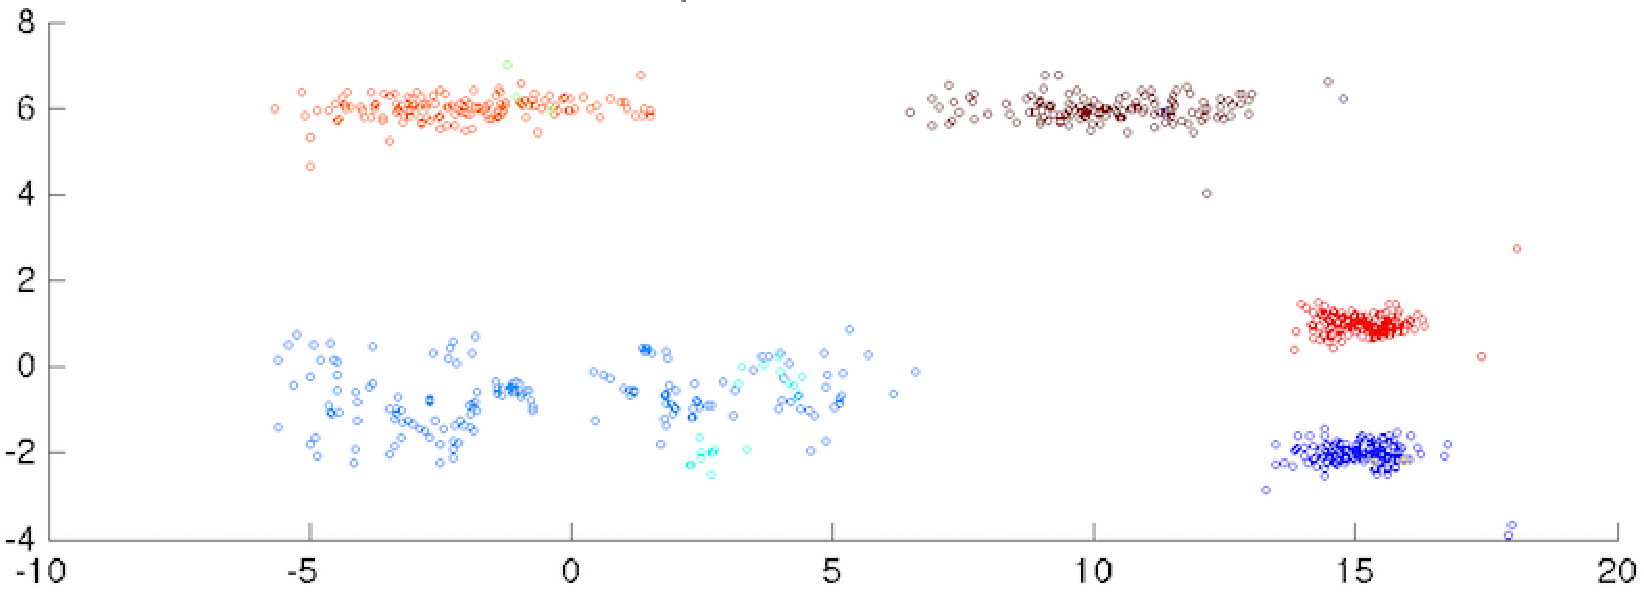
\includegraphics[scale=0.5]{toy_example_after_Dsnn_1.pdf}
  \caption{Toy example: Data after distributed snn clustering with $Eps=60$.}
  \label{fig:toy_dsnn2}
\end{figure}



\section{Methodology and Experimental results}
In this section, we assess the performance of the proposed distributed algorithm and contrasts its effectiveness against a centralized version and against an efficient and widely used SNN-graph bisection method\cite{ZK02}, both of them use the complete dataset loaded into main memory.
% se podrian presentar brevemente los métodos con que se comparará
% se podria introducir aqui los hallazgos que encontramos luego de los experimentos.

Initially, a proof of concept was made by applying the algorithm over the synthetic dataset shown in figure \ref{fig:toy_original} which was proposed by \cite{GRS98}. Since this dataset contains points in two dimensions, the discriminative capability of the proposal in presence of  high dimensional data is not assessed. In spite of that, the effectiveness of the distributed algorithm and its robustness to noise in the data are evaluated in a qualitative fashion. The obtained clusters in two independent runs with different parameters are depicted in figures \ref{fig:toy_dsnn1} and \ref{fig:toy_dsnn2}.

%comentarios de los resultados
By contrasting figure \ref{fig:toy_original} against \ref{fig:toy_dsnn1} and then against figure \ref{fig:toy_dsnn2}, it is noticed that the noise layer was removed by the clustering algorithm in both cases. Additionally, the increase in the Eps value had an impact onto the sensitivity of the algorithm to detect outliers, i.e. a higher value for this parameter was accompanied by an increasing rate of points marked as noise as it is specially noticed in the chain of outliers that connects the two ellipsoids in figure \ref{fig:toy_original}.

\subsection*{Datasets}
The experiments were performed over 5 collections containing documents represented as vectors in high dimensional term spaces. By following the descriptions shown in table \ref{table:datasets}, firstly the 20-Newsgroup (M5 partition) collection contains $5000$ newsgroup documents coming from different subjects, namely computers, motorcycles, baseball, science and politics. Then, the remaining document sets were extracted from the Tipster collection\footnote{\url{https://tac.nist.gov/data/data_desc.html#TIPSTER} (Last visit on November 8th, 2016.)} and comprise several heterogeneous datasets such as \textit{DOE} which contains short abstracts of the Department of Energy, and \textit{FR} which contains reports of actions taken by U.S. government agencies.
Also in table \ref{table:datasets}, the number of documents, the size of the vocabulary, the number of classes and the percentage of non zero values (a measure of the sparsity of the collection) are shown. As a final remark, all collections are quite sparse and also their document vectors are spanned onto high dimensional term spaces with tens of thousands of features. 

In each one of the subfigures appearing in the Figure \ref{fig:sim_matrices}, similarities between all pair of documents in each collection are plotted by using a gray scale. Darker spots denote higher similarity values and also the documents were ordered consecutively by the group label. In all the figures, both axes contain the document numbers (starting from $0$) and, regarding the previously mentioned document order, it is possible to observe the groups denoted as darker rectangular patches along the diagonal line.

From the Figure \ref{fig:sim_matrices}, it is possible to observe the following patterns in the similarity matrices: 
First, 20NG and ZF collections show pairwise intra-similarities not much higher than the ones outside the groups. Also, in the case of the DOE collection, some spots outside the diagonal appear which suggests the existence of groups not registered in the original labelings.
Finally, the matrices of the FR and SJMN collections show small squares embedded into the bigger squares along the diagonal which suggests the existence of a hierarchical structure underlying both document sets.

\begin{table}[htbp]
\centering
\noindent\adjustbox{max width=\textwidth}{%
\begin{tabular}{llrrrc}
    \hline
    Dataset & Description &instances & $|\set{V}|$ & classes & $\pct$NNZ\\ \hline
\textit{20NG} & 20-newsgroup data, m5 partition. & $4743 $ & $41223$ & $5$   & $0.167\pct$ \\     
\textit{DOE} &  Department of Energy Abstracts& $1664$ & $15755 $ & $14$     & $0.365\pct$ \\ 
\textit{FR} & Federal Register notes& $926 $ & $50427 $ & $14$               & $1.104\pct$ \\ 
\textit{SJMN} & San Jose Mercury News & $908 $ & $23616$ & $16$              & $0.738\pct$ \\ 
\textit{ZF} & Computer select disks by Ziff-Davis & $3263 $ & $58398 $ & $25$& $0.360\pct$ \\ \hline % end of tipster.
\end{tabular}}
\caption{Datasets employed.}
\label{table:datasets}
\end{table}

%%% GRAFICOS DE SIMILITUD
\begin{figure}[!htbp]
    \centering
    \begin{subfigure}[b]{0.3\textwidth}
        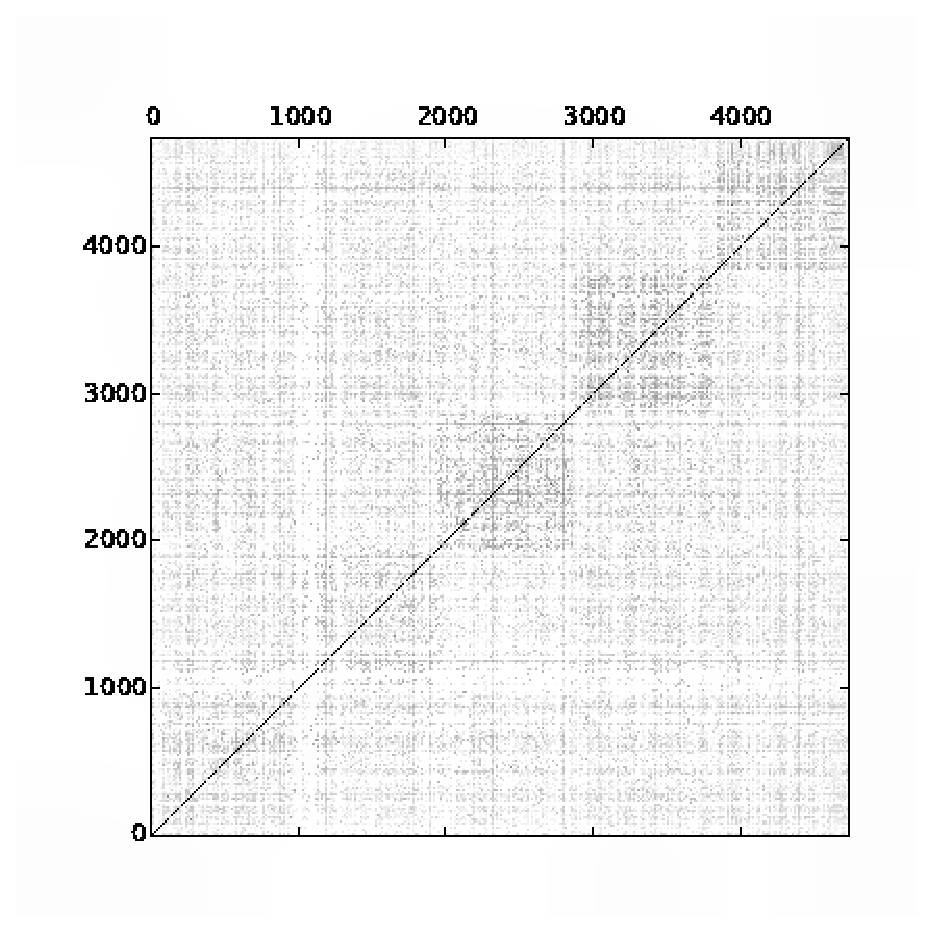
\includegraphics[width=\textwidth]{./similarities/20NG-simcos}
        \caption{The 20NG collection.}
        \label{fig:20ng_sim}
    \end{subfigure}
    ~ %add desired spacing between images, e. g. ~, \quad, \qquad, \hfill etc. 
      %(or a blank line to force the subfigure onto a new line)
    \begin{subfigure}[b]{0.3\textwidth}
        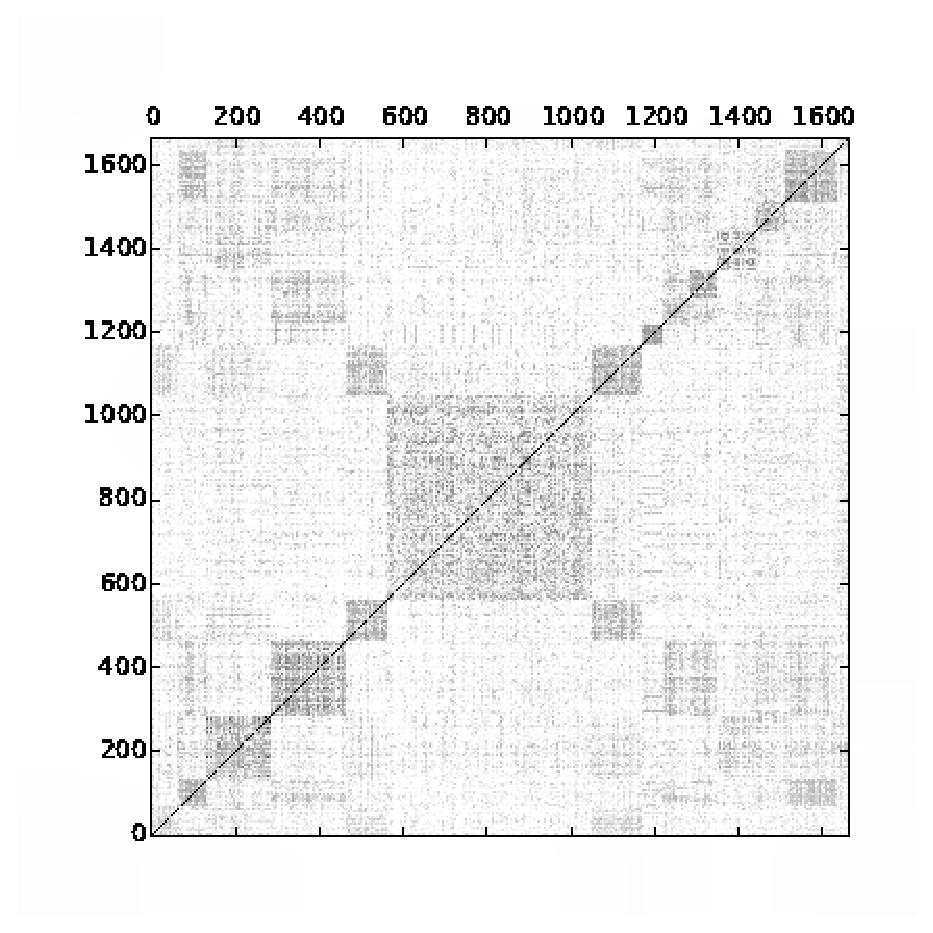
\includegraphics[width=\textwidth]{./similarities/DOE-simcos}
        \caption{The DOE collection.}
        \label{fig:doe_sim}
    \end{subfigure}\\
    
    \begin{subfigure}[b]{0.3\textwidth}
        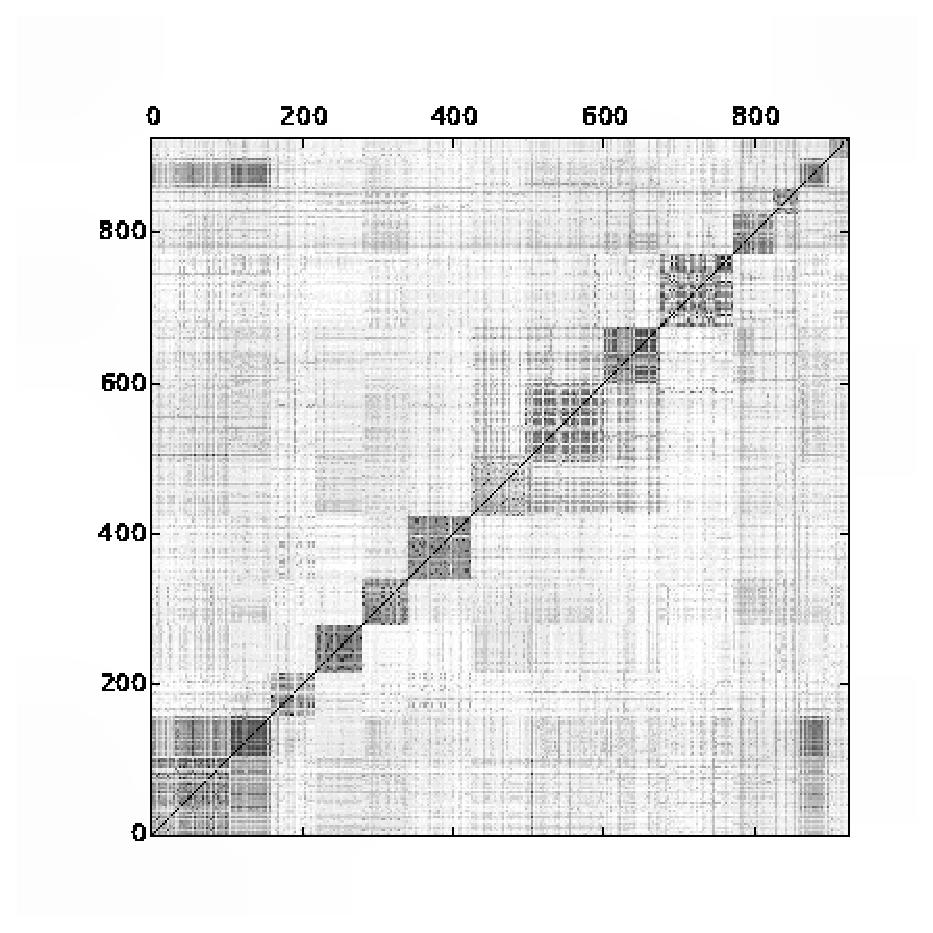
\includegraphics[width=\textwidth]{./similarities/FR-simcos}
        \caption{The FR collection.}
        \label{fig:fr_sim}
    \end{subfigure}
    ~ %add desired spacing between images, e. g. ~, \quad, \qquad, \hfill etc. 
      %(or a blank line to force the subfigure onto a new line)
    \begin{subfigure}[b]{0.3\textwidth}
        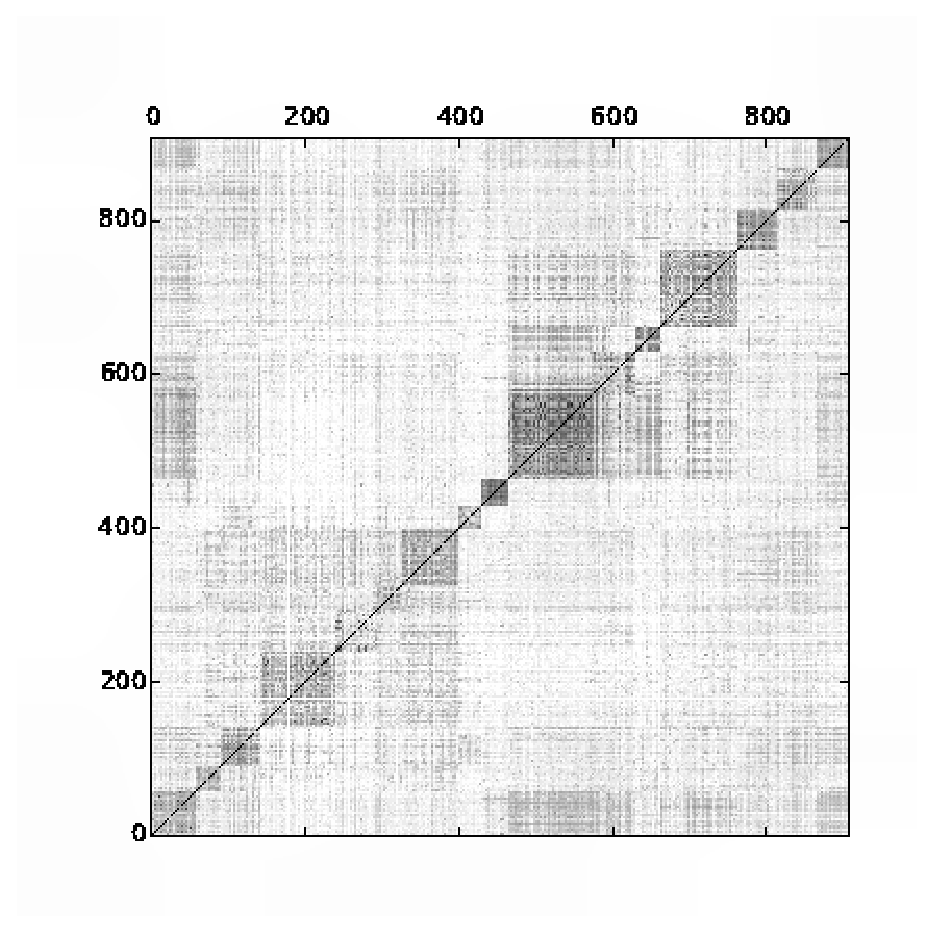
\includegraphics[width=\textwidth]{./similarities/SJMN-simcos}
        \caption{The SJMN collection.}
        \label{fig:sjmn_sim}
    \end{subfigure}\\
        
    \begin{subfigure}[b]{0.3\textwidth}
        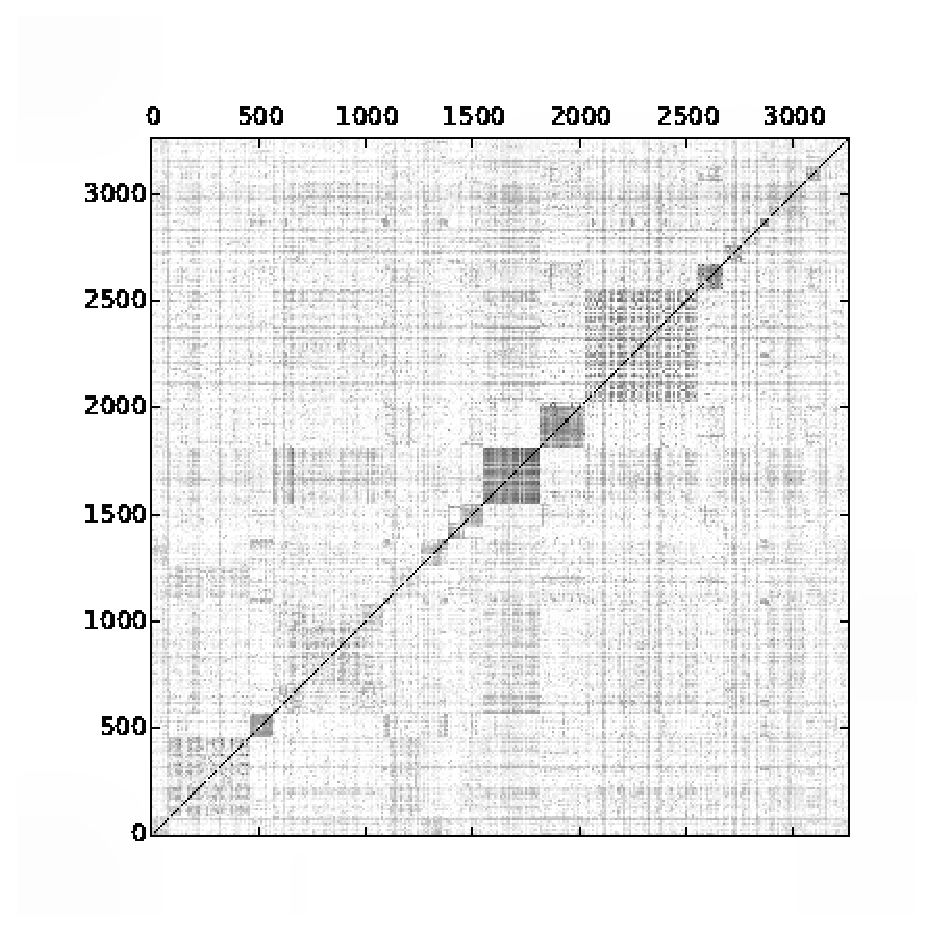
\includegraphics[width=\textwidth]{./similarities/ZF-simcos}
        \caption{The ZF collection.}
        \label{fig:zf_sim}
    \end{subfigure}    
    \caption{Pairwise cosine-similarity matrices}\label{fig:sim_matrices}
\end{figure}

\subsubsection*{Document processing}
To obtain a representative set of terms for each collection, i.e. its index terms, the documents are preprocessed as it is depicted in figure \ref{fig:text_processing}. This figure shows  standard text processing steps commonly used in Information retrieval and text clustering tasks. Firstly, as documents within the Tipster collections come in SGML format, their content is extracted. Then, spacing and punctuation marks are removed in order to keep only the candidate terms of the vocabulary. After this step, the set of candidate terms is filtered by using a standard English stopword set, which aids to remove meaningless words (e.g. articles) and some highly frequent words. No other ad-hoc filter is applied to the documents in this work (e.g. stemming or removing very high and low frequency words) in order to keep the text content as similar as possible to the original version and specially to allow subsequent generalizations of the performance results of the proposal without any tie to a specific dataset. Finally, the selected terms within each collection are sorted and then the index term set or vocabulary is obtained.

After the vocabulary of each collection is built, the number of occurrences of its terms in each document are computed and used to build the vector representing each document. That is, the number of occurrences of a term $i$ of the  vocabulary $\mathcal{V}$ in the document $j$ of the collection is denoted as $f_{i,j}$, also the number of documents of the collections that contain this term is denoted as $N_{i}$. By following this notation, the weight of term $i$ within a document $j$ is quantified by the expression:\[w_{i,j}=\frac{f_{i,j}}{ \operatorname*{max}_{t\in \mathcal{V}}f_{t,j} }\cdot\log\frac{|\mathcal{V}|}{N_{i}}\] In this way, the vector representing document $j$ is made up by the weight of each term of the vocabulary in it.

\subsection*{Clustering quality measures}
In this work, only external validation measures are employed, namely \textbf{Entropy}, \textbf{Purity}, \textbf{Adjusted-Rand-Index}, \textbf{Adjusted-Mutual-Information}, \textbf{Homogeneity}, \textbf{Completeness} and the \textbf{V-Measure} which consists in the harmonic mean between the Homogeneity and Completeness scores. These scores, with the exception of  the Adjusted-Rand-Index which is within $[-1,1]$,  have positive values within $[0,1]$. Also, with the exception of Entropy, for all of them larger values denote a better clustering quality.

\textbf{Entropy}, measures the extent in which all data from one class are spread into several groups and 
\textbf{Purity} measures the extent that a cluster contains only one class of data. 
\textbf{Adjusted-Rand-Index} measures the matching between the true labels and the ones produced by the algorithm under study by counting the proportion of point-pairs whose relationship is the same in both labelings.
\textbf{Adjusted-Mutual-Information}  accounts for the matching level between two clusterings by measuring the amount of information shared between the true labeling and the one proposed by an algorithm. Both scores are adjusted because of the original estimates are higher for two clusterings with a larger number of clusters, regardless of whether there is actually more information shared between them.
\textbf{Homogeneity} measures the extent in which the clusters contain only data points which are members of a single class. 
\textbf{Completeness} accounts for the extent in which all the data points that are members of a given class are elements of the same cluster.


\subsection*{Parameter tuning}
In order to report the best performance found for each algorithm, its parameters must be tuned.
Hence, for each algorithm a grid search is performed seeking the parameter values that allow to attain the best algorithm performance. The parameter grid used for the Centralized and Distributed SNN clustering algorithms consists of $288$ configurations where the values of $K$ are in $\{50, 70, 90, 110\}$, $\mathsf{Eps}$ are in $\{3, 5, 8, 10, 15, 20, 25, 30, 35, 40, 45, 50\}$ and $\mathsf{MinPts}$ are in $\{5, 10, 15, 20, 25, 30\}$. For the SNN-Graph bisection algorithm the same values for $K$ were tested but no difference in the performance was detected. In Tables \ref{table:centralizedsnn_params} and \ref{table:distributedsnn_params} the parameters chosen  after the tuning procedure are detailed.

\begin{figure}[!htbp]
\centering
  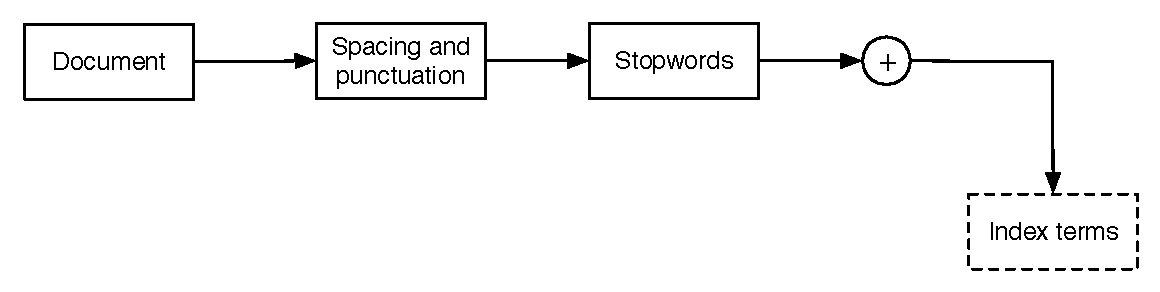
\includegraphics[scale=0.7]
  {text_processing_steps.pdf}
  \caption{Text processing steps performed in each collection.}
  \label{fig:text_processing}
\end{figure}


\begin{table}[!htbp]
\centering
\begin{tabular}{l|crr}
\textbf{Dataset} & \textbf{K} & \textbf{Eps} & \textbf{MinPts} \\ \hline
20NG    & 110& 25 & 30 \\
DOE     &  70& 25 & 30 \\
FR      &  50& 25 & 20  \\
SJMN    &  50& 20 & 30 \\
ZF      &  90& 40 & 25 \\ \hline
\end{tabular}
\caption{Parameters of the centralized SNN-Clustering algorithm selected after the tuning procedure.}
\label{table:centralizedsnn_params}
\end{table}


\begin{table}[!htbp]
\centering
\begin{tabular}{l|crr}
\textbf{Dataset} & \textbf{K} & \textbf{Eps} & \textbf{MinPts} \\ \hline
20NG    & 30& 8 & 25 \\
DOE     & 30& 10& 20 \\
FR      & 30& 10& 5  \\
SJMN    & 30& 10& 10 \\
ZF      & 30& 10& 15 \\ \hline
\end{tabular}
\caption{Parameters of the distributed SNN-Clustering algorithm selected after the tuning procedure.}
\label{table:distributedsnn_params}
\end{table}


\subsection*{Results}
The results shown in Table \ref{table:results} demonstrate that the distributed SNN attains a comparable performance to the other two algorithms which also attained acceptable results. In most cases the proposal achieved better scores, nevertheless it is important to mention that a potential improvement is possible for the graph clustering algorithm by applying a better tuning strategy. 

%comentar dificultad de los conjuntos de datos

%

% HOM y COM
20NG and ZF datasets presented more difficulties to the centralized algorithms in terms of identifying homogeneous clusters (include only the points from a given class within a cluster), especially to the C-SNN algorithm. In contrast, the D-SNN performed in a stable manner along all the datasets attaining generally higher scores. This suggests that it is able to  overcome the weakness of its centralized relative when it faces data having low contrast between intra-group and extern pairwise similarities. 

%HOM : class distribution within each cluster should be skewed to a single class. (Incluye solamente los puntos de la clase en el cluster)
%COM : the distribution of cluster assignments within each class should be completely skewed to a single cluster. (Incluye todos los puntos de la clase)

% variabilidad de los centralizados en sus desempeños
% costos computacionales debido a al computo secuencial del algorutmo y calculo de matrices de similitud

\begin{table}[!htbp]
\centering
\begin{tabular}{cl|cllllll}
%ARI(3) AMI(4) NMI(5) HOM(6) COM(7) VMea(8)
&\textbf{Dataset} & \textbf{Entropy} & \textbf{Purity} & \textbf{ARI} & \textbf{AMI}  & \textbf{HOM} & \textbf{COM} & \textbf{VM} \\ \hline
%CLUTO
\parbox[t]{2mm}{\multirow{5}{*}{\rotatebox[origin=c]{90}{Graph Clust}}} &20NG    & 0.2948 &  0.8307 &  0.6050 &  0.6421 &  0.6619 &  0.6425 &  0.6521  \\
&DOE     & 0.2721 &  0.7139 &  0.4919 &  \textbf{0.7030}  &  0.7095 &  \textbf{0.7461} &  0.7273  \\
&FR        & 0.2524 &  0.7559 &  0.6185 &  0.7266   &  0.7375 &  0.7452 &  0.7413  \\
&SJMN   & 0.2412 &  0.7544 &  0.5953 &  0.7367 &  0.7505 &  0.7657 &  0.7580  \\
&ZF        & 0.4166 &  0.6028 &  0.3817 &  0.5444 &  0.5593 &  0.6015 &  0.5796  \\ \hline
% CENTRALIZED
\parbox[t]{2mm}{\multirow{5}{*}{\rotatebox[origin=c]{90}{C-SNN}}} &20NG    & 0.3525 & 0.6036 & 0.3432 & 0.3953 & 0.3990 & 0.4793 & 0.4355\\
&DOE     & 0.2865 & 0.6911 & 0.4197 & 0.6370 &  0.6476 & 0.6711 & 0.6591\\
&FR        & 0.1921 & 0.8531 & 0.7099 & \textbf{0.7834} &  0.7969 & 0.7919 & 0.7944\\
&SJMN   & 0.2024 & \textbf{0.8282} & 0.5846 & 0.6820 & 0.7732 & 0.6960 & 0.7326\\
&ZF        & 0.3330 & 0.6089 & 0.2845 & 0.5084 &  0.5750 & 0.5238 & 0.5482\\ \hline
%DISTRIB
\parbox[t]{2mm}{\multirow{5}{*}{\rotatebox[origin=c]{90}{D-SNN}}} &20NG    & \textbf{0.1710} & \textbf{0.8828} & \textbf{0.8400} & \textbf{0.8218} & \textbf{0.8262} & \textbf{0.9167} & \textbf{0.8691}  \\
&DOE     & \textbf{0.1074} & \textbf{0.9318} & \textbf{0.6816} & 0.7029  &  \textbf{0.8794} & 0.7227 & \textbf{0.7934}  \\
&FR        & \textbf{0.0949} & \textbf{0.9134} & \textbf{0.7224} & 0.7546  & \textbf{0.8947} & \textbf{0.7784} & \textbf{0.8325}  \\
&SJMN   & \textbf{0.1802} & 0.7656 & \textbf{0.6360} & \textbf{0.7836}  & \textbf{0.8052} & \textbf{0.8040} & \textbf{0.8046}  \\
&ZF        & \textbf{0.0117} & \textbf{0.9943} & \textbf{0.7809} & \textbf{0.7701}   & \textbf{0.9882} & \textbf{0.7877} & \textbf{0.8766}  \\ \hline
\end{tabular}
\caption{Performance attained by the graph clustering algorithm, the centralized SNN algorithm and the  distributed proposal  over the text collections. The best values for each measure in each dataset appear in bold face.}
\label{table:results}
\end{table}



\section{Conclusions and future work}
In this work, the hypothesis consists in that the proposal is able to deal with distributed text collections and then to recover the group structure underlying the whole dataset with a quality comparable to centralized algorithms successfully used in the clustering literature.


%% OJO  CON ESTA FRASE ...
Beyond the labeling of each data point, the task that we found more important specially in BIgData scenarios is the cluster recovery task. Its aim is to summarize a data collection by reconstructing the group structure underlying the set of data points.






\section{Acknowledgment}
Juan Zamora was supported by an intern postdoc project from Pontificia Universidad Cat\'olica de Valpara\'iso.
\clearpage 

\bibliographystyle{apalike}
% \bibliography{references}
\begin{thebibliography}{}

\bibitem[Bahmani et~al., 2012]{BMVKV12}
Bahmani, B., Moseley, B., Vattani, A., Kumar, R., and Vassilvitskii, S. (2012).
\newblock {Scalable K-Means ++}.
\newblock {\em Proceedings of the VLDB Endowment (PVLDB)}, 5:622--633.

\bibitem[Balcan et~al., 2013]{BEL13}
Balcan, M.~F., Ehrlich, S., and Liang, Y. (2013).
\newblock {Distributed k -Means and k -Median Clustering on General
  Topologies}.
\newblock {\em Advances in Neural Information Processing Systems 26 (NIPS
  2013)}, pages 1--9.

\bibitem[Crestani and Markov, 2013]{CM13}
Crestani, F., and Markov, I. (2013).
\newblock {Distributed Information Retrieval and Applications}.
\newblock {\em 35th European Conference on IR Research}, 865--868.

\bibitem[Das et~al., 2007]{DDGR07}
Das, A., Datar, M., Garg, A., and Rajaram, S. (2007).
\newblock Google news personalization: scalable online collaborative filtering.
\newblock In {\em Proceedings of the 16th international conference on World
  Wide Web}, pages 271--280. ACM.

\bibitem[De~Vries et~al., 2015]{VVGN15}
De~Vries, C.~M., De~Vine, L., Geva, S., and Nayak, R. (2015).
\newblock Parallel streaming signature {EM}-tree: A clustering algorithm for web
  scale applications.
\newblock In {\em Proceedings of the 24th International Conference on World
  Wide Web}, pages 216--226. ACM.

\bibitem[Dhillon and Modha, 1999]{DM99}
Dhillon, I.~S. and Modha, D.~S. (1999).
\newblock {A data-clustering algorithm on distributed memory multiprocessors}.
\newblock {\em LargeScale Parallel Data Mining}, 1759(802):245--260.

\bibitem[Ene et~al., 2011]{EIM11}
Ene, A., Im, S., and Moseley, B. (2011).
\newblock {Fast Clustering using MapReduce}.
\newblock {\em Kdd}, 681--689.

\bibitem[Ert{\"o}z et~al., 2003]{ESK03}
Ert{\"o}z, L., Steinbach, M., and Kumar, V. (2003).
\newblock {Finding clusters of different sizes, shapes, and densities in noisy, high dimensional data}.
\newblock {\em Proceedings of the SIAM International Conference on Data Mining}, 47--58.

% \bibitem[Ester et~al., 1996]{EKSX96}
% Ester, M., Kriegel, H., Sander, J., and Xu, X. (1996)
% \newblock {A density-based algorithm for discovering clusters in large spatial databases with noise}.
% \newblock {\em Proceedings of the Second International Conference on Knowledge Discovery and Data Mining}, 96:226--231.

\bibitem[Forman and Zhang, 2000]{FZ00}
Forman, G. and Zhang, B. (2000).
\newblock {Distributed data clustering can be efficient and exact}.
\newblock {\em ACM SIGKDD Explorations Newsletter}, 2(2):34--38.

\bibitem[Guha et~al., 1998]{GRS98}
Guha, S., Rastogi, R. and Shim, K. (1998).
\newblock{CURE: an efficient clustering algorithm for large databases}.
\newblock{\em ACM SIGMOD Record},  27(2):73--84.

\bibitem[Han et~al., 2011]{HK11}
Han, J., Pei, J., and Kamber, M. (2011).
\newblock {\em Data mining: concepts and techniques}.
\newblock Elsevier.

\bibitem[Indra et~al., 2014]{I14}
Indra, Z., Zamin, N., Jaafar, J. (2014).
\newblock{A clustering technique using single pass clustering algorithm for search engine}.
\newblock{\em 2014 4th World Congress on Information and Communication Technologies (WICT 2014)},  1:182--187.

\bibitem[Jagannathan et~al., 2005]{JW05}
Jagannathan, G., and Wright, R. N. (2005).
\newblock {Privacy-preserving Distributed K-means Clustering over Arbitrarily Partitioned Data}.
\newblock {\em Proceedings of the Eleventh ACM SIGKDD International Conference on Knowledge Discovery in Data Mining}, 593--599.

\bibitem[Januzaj et~al., 2003]{JKP03}
Januzaj, E., Kriegel, H.-P., and Pfeifle, M. (2003).
\newblock {Towards Effective and Efficient Distributed Clustering}.
\newblock {\em Workshop on Clustering Large Data Sets}, pages 49--58.

\bibitem[Januzaj et~al., 2004]{JKP04}
Januzaj, E., Kriegel, H.-P., and Pfeifle, M. (2004).
\newblock {Scalable Density-Based Distributed Clustering}.
\newblock pages 231--244.

\bibitem[Jin et~al., 2015]{JCHAC15}
Jin, C., Chen, Z., Hendrix, W., Agrawal, A., and Choudhary, A. (2015).
\newblock {Incremental, Distributed Single-linkage Hierarchical Clustering
  Algorithm Using Mapreduce}.
\newblock {\em Proceedings of the Symposium on High Performance Computing},
  pages 83--92.

\bibitem[Johnson and Kargupta, 2000]{JK00}
Johnson, E. and Kargupta, H. (2000).
\newblock {Collective, hierarchical clustering from distributed, heterogeneous
  data}.
\newblock {\em Lecture Notes in Computer Science}, 1759:221--244.

\bibitem[Kargupta et~al., 2001]{KHSJ01}
Kargupta, H., Huang, W., Sivakumar, K., and Johnson, E. (2001).
\newblock Distributed clustering using collective principal component analysis.
\newblock {\em Knowledge and Information Systems}, 3(4):422--448.

\bibitem[Klusch et~al., 2003]{KLM03}
Klusch, M., Lodi, S., and Moro, G. (2003).
\newblock {Distributed clustering based on sampling local density estimates}.
\newblock {\em IJCAI International Joint Conference on Artificial
  Intelligence}, pages 485--490.

\bibitem[Kriegel et~al., 2005]{KKPS05}
Kriegel, H.-p., Kr, P., Pryakhin, A., and Schubert, M. (2005).
\newblock {Effective and Efficient Distributed Model-based Clustering}.

\bibitem[Li et~al., 2003]{LZO03}
Li, T., Zhu, S., and Ogihara, M. (2003).
\newblock {Algorithms for Clustering High Dimensional and Distributed Data}.
\newblock {\em Intelligent Data Analysis Journal}, 7(February):1--36.

\bibitem[Liang et~al., 2013]{LBK13}
Liang, Y., Balcan, M.-f., and Kanchanapally, V. (2013).
\newblock {Distributed PCA and k-Means Clustering}.
\newblock {\em The Big Learning Workshop in NIPS 2013}, pages 1--8.

\bibitem[Liu et~al., 2012]{LHLX12}
Liu, J., Huang, J. Z., Luo, J., and Xiong, L. (2012).
\newblock {Privacy Preserving Distributed DBSCAN Clustering}.
\newblock {\em Proceedings of the 2012 Joint EDBT/ICDT Workshops}, 177--185.


\bibitem[Merugu and Ghosh, 2003]{MG03}
Merugu, S. and Ghosh, J. (2003).
\newblock {Privacy-preserving Distributed Clustering using Generative Models}.
\newblock {\em Proceedings of the 3rd IEEE International Conference on Data
  Mining (ICDM)}, pages 0--7.

\bibitem[Nagwani, 2015]{N15}
Nagwani, N. K. (2015).
\newblock {Summarizing large text collection using topic modeling and clustering based on MapReduce framework}.
\newblock {\em Journal of Big Data}, 2:1--18.

\bibitem[Naldi and Campello, 2014]{NC14}
Naldi, M.~C. and Campello, R. J. G.~B. (2014).
\newblock {Evolutionary k-means for distributed data sets}.
\newblock {\em Neurocomputing}, 127:30--42.

\bibitem[Qi et~al., 2008]{ZLW08}
Qi, Z., Jinze, L., and Wei, W. (2008).
\newblock {Approximate clustering on distributed data streams}.
\newblock {\em Proceedings - International Conference on Data Engineering},
  00:1131--1139.

\bibitem[Rousseeuw, 1987]{R87}
Rousseeuw Peter J. (1987). 
\newblock {Silhouettes: A graphical aid to the interpretation and validation of cluster analysis}.
\newblock {\em Journal of Computational and Applied Mathematics}, 20:53--65.

\bibitem[Sarnovsky et~al, 2016]{SC16}
Sarnovsky, M., Carnoka, N.. (2016). 
\newblock {Distributed Algorithm for Text Documents Clustering Based on k-Means Approach}.
\newblock {\em Advances in Intelligent Systems and Computing}, 430:165--174.

\bibitem[WWWSize, 2016]{www}
http://www.worldwidewebsize.com/
Accessed at 26th September 2016

\bibitem[Xu et~al., 1999]{XJK99}
Xu, X., J{\"{a}}ger, J., and Kriegel, H. (1999).
\newblock {A fast parallel clustering algorithm for large spatial databases}.
\newblock {\em High Performance Data Mining}, 290:263--290.

\bibitem[Yi et~al., 2014]{Yi14}
Yi, J., ZShang, L., Wang, J., Jin, R., Jain, A.K. (2014)
\newblock {A Single-Pass Algorithm for Efficiently Recovering Sparse Cluster Centers of High-dimensional Data}.
\newblock {\em Proceedings of the 31 st International Conference on Machine
Learning, Beijing, China, 2014.}, 3:2112--2127.

\bibitem[Zhang et~al., 2013]{ZW13}
Zhang, J., Wu, G., Hu, X., Li, S., Hao, S. (2013).
\newblock{A Parallel Clustering Algorithm with MPI – MKmeans }.
\newblock{\em Jouirnal of Computers}, 8(1):10--18.

\bibitem[Zhao et~al., 2002]{ZK02}
Zhao, Y. and Karypis, G. (2002).
\newblock{Evaluation of hierarchical clustering algorithms for document datasets}.
\newblock{\em Proceedings of the eleventh international conference on Information and knowledge management}, 515--524.


\end{thebibliography}
\end{document}